\documentclass[fleqn, a4paper, 11pt, oneside]{amsart}
%\usepackage[top = 2cm, bottom = 1cm, left = 1cm, right = 1cm]{geometry}
\usepackage{exsheets, tasks}
\usepackage{amsmath, amssymb, amsthm} %standard AMS packages
\usepackage{marginnote} %marginnotes
\usepackage{gensymb} %miscellaneous symbols
\usepackage{commath} %differential symbols
\usepackage{xcolor} %colours
\usepackage{cancel} %cancelling terms
\usepackage[free-standing-units, space-before-unit]{siunitx} %formatting units
	\sisetup
	{
		per-mode=fraction,
		fraction-function=\frac
	}
\usepackage{tikz, pgfplots} %diagrams
\usetikzlibrary{calc, hobby, patterns, intersections, decorations.markings}
\usepackage{graphicx} %inserting graphics
\usepackage{hyperref} %hyperlinks
\usepackage{datetime} %date and time
\usepackage{ulem} %underline for \emph{}
\usepackage{xfrac} %inline fractions
\usepackage{enumerate,enumitem} %numbered lists
\usepackage{float} %inserting floats
\usepackage{circuitikz}[american voltages, american currents] %circuit diagrams
\usepackage[utf8]{inputenc}
\usepackage{booktabs}
\usepackage{todonotes}

\newcommand\numberthis{\addtocounter{equation}{1}\tag{\theequation}} %adds numbers to specific equations in non-numbered list of equations

\newcommand{\AxisRotator}[1][rotate=0]{
	\tikz [x=0.25cm,y=0.60cm,line width=.2ex,-stealth,#1] \draw (0,0) arc (-150:150:1 and 1);%
} %rotation symbols on axes

\theoremstyle{definition}
\newtheorem{example}{Example}
\newtheorem{definition}{Definition}

\theoremstyle{theorem}
\newtheorem{theorem}{Theorem}

\newcommand{\curl}{\mathrm{curl\,}}

\makeatletter
\@addtoreset{section}{part} %resets section numbers in new part
\makeatother

\renewcommand{\thesubsection}{(\arabic{subsection})}
\renewcommand{\thesection}{(\arabic{section})}

\renewcommand{\emph}{\uline}

\renewcommand{\tilde}{\widetilde}

%section headings on left
\makeatletter
\def\specialsection{\@startsection{section}{1}%
	\z@{\linespacing\@plus\linespacing}{.5\linespacing}%
	%  {\normalfont\centering}}% DELETED
	{\normalfont}}% NEW
\def\section{\@startsection{section}{1}%
	\z@{.7\linespacing\@plus\linespacing}{.5\linespacing}%
	%  {\normalfont\scshape\centering}}% DELETED
	{\normalfont\scshape}}% NEW
\makeatother

%forces newline after subsection
\makeatletter
\def\subsection{\@startsection{subsection}{3}%
	\z@{.5\linespacing\@plus.7\linespacing}{.1\linespacing}%
	{\normalfont\itshape}}
\makeatother

\settasks{counter-format = tsk[1].}

\SetupExSheets{solution/print = true}

%opening
\title{Quantum and Solid State Physics : Assignment 10}
\author
{
	Aakash Jog\\
	ID : 989323563
}
\date{\formatdate{31}{12}{2015}}

\begin{document}

\tikzset{->-/.style={decoration={
  markings,
  mark=at position #1 with {\arrow{>}}},postaction={decorate}}}

\maketitle
%\setlength{\mathindent}{0pt}

\begin{question}
	Consider two silicon samples at room temperature, doped P-type with $N_A = 10^{16} \si{\per\centi\metre\cubed}$.
	Light shines on the left side of the sample, such that a steady state excess carrier concentration of $10^{14} \si{\per\centi\metre\cubed}$ is maintained at $x = 0$, and $G_{\text{optical}} = 0$, throughout the rest of the sample.\\
	Sample 1 is short and has a metal contact at $x = L_1 << L_n$.\\
	Sample 2 is short and has a metal contact at $x = L_2 >> L_n$.
	\begin{enumerate}
		\item
			For both samples, which of the following shows the correct directions of electron diffusion and electron diffusion current density $J_{\text{diffusion}_n}$ in the samples.
			\begin{enumerate}
				\item
					\begin{tabular}{l l l l}
						electron diffusion & $\rightarrow$ & $J_{\text{diffusion}_n}$ & $\rightarrow$\\
					\end{tabular}
				\item
					\begin{tabular}{l l l l}
						electron diffusion & $\rightarrow$ & $J_{\text{diffusion}_n}$ & $\leftarrow$\\
					\end{tabular}
				\item
					\begin{tabular}{l l l l}
						electron diffusion & $\leftarrow$ & $J_{\text{diffusion}_n}$ & $\rightarrow$\\
					\end{tabular}
			\end{enumerate}
		\item
			If $10^{19}$ EHPs are generated per second, i.e. $G_{\text{optical}} = 10^{19} \si{\per\centi\metre\cubed\per\second}$, calculate the minority carrier lifetime in $\si{\micro\second}$.
		\item
			On the same axes, plot $n(x)$, the minority carrier concentration, in both samples, as a function of position.
		\item
			If the length of sample 1 is one hundredth of the elecetron diffusion length, i.e.
			\begin{align*}
				L_n & = 100 L_1
			\end{align*}
			whet is the correct expression for electron current density, $J_{\text{diffusion}_n}(x)$?
			\begin{enumerate}
				\item $J_{\text{diffusion}_n}(x) = -100 q G_{\text{optical}} L_n e^{-\frac{x}{L_n}}$
				\item $J_{\text{diffusion}_n}(x) = -100 q G_{\text{optical}} {L_n}^2$
				\item $J_{\text{diffusion}_n}(x) = -\frac{1}{100} q G_{\text{optical}} L_n$
				\item $J_{\text{diffusion}_n}(x) = -100 q G_{\text{optical}} L_n$
			\end{enumerate}
		\item
			For sample 2, what is the electron diffusion current density at $x = 0$?
			\begin{enumerate}
				\item $J_{\text{diffusion}_n}(x = 0) = -q G_{\text{optical}} L_n$
				\item $J_{\text{diffusion}_n}(x = 0) = -100 q G_{\text{optical}} L_n$
				\item $J_{\text{diffusion}_n}(x = 0) = -\frac{1}{100} q G_{\text{optical}} L_n$
			\end{enumerate}
		\item
			On the same axes, plot the magnitude of electron diffusion current density $\left| J_{\text{diffusion}_n}(x) \right|$ in both samples as a function of position.
	\end{enumerate}
\end{question}

\begin{solution}
	\begin{enumerate}[leftmargin=*]
		\item
			As the samples are illuminated on the left only, there is an excess of electrons on the left, as compared to the right.
			Therefore, \emph{the direction of electron diffusion will be $\rightarrow$}, and hence, \emph{the direction of $J_{\text{diffusion}_n}$ will be $\leftarrow$}.
		\item
			\begin{align*}
				\hat{n}            & = G_{\text{optical}} \tau_p \\
				\therefore 10^{14} & = 10^{19} \tau_p            \\
				\therefore \tau_p  & = 10^{-5} \si{\second}      \\
				\therefore \tau_p  & = 10 \si{\micro\second}
			\end{align*}
		\item
			\begin{figure}[H]
				\centering
				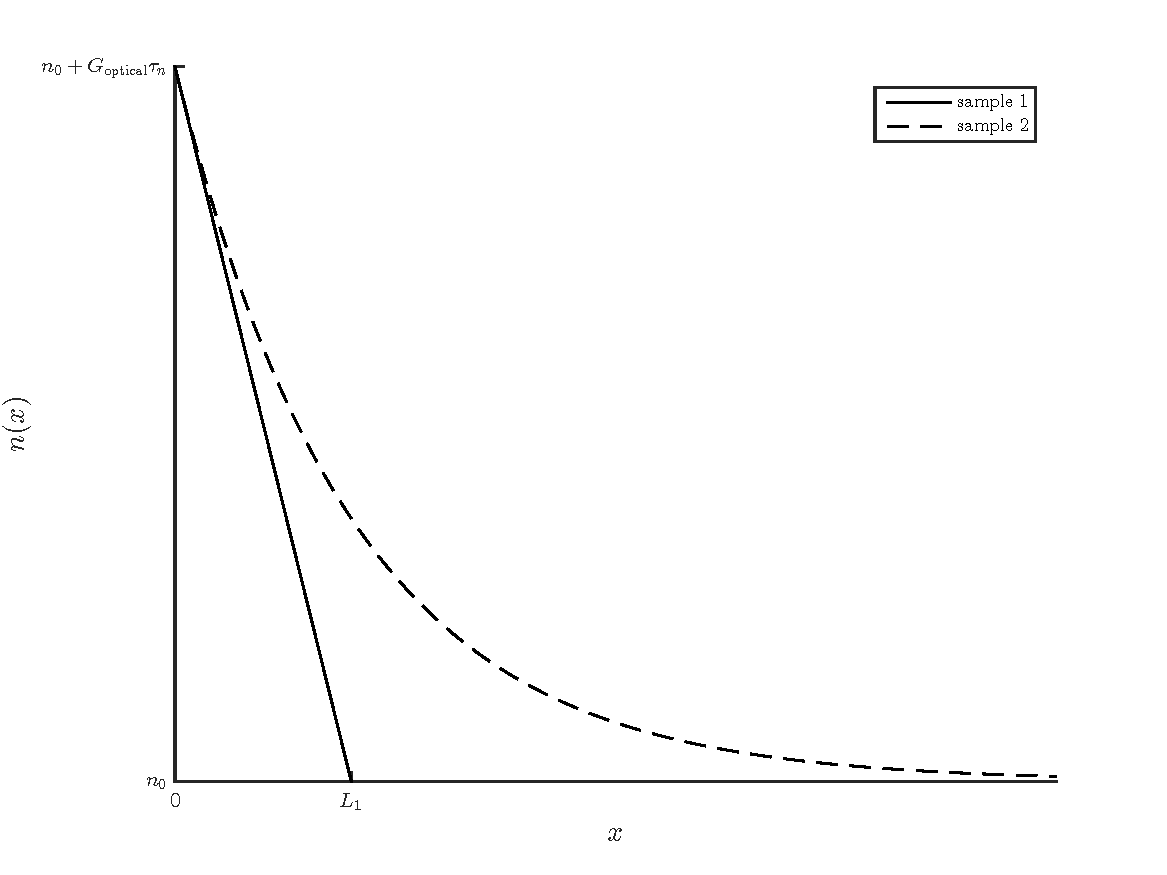
\includegraphics[width = 0.8\textwidth]{plot1.pdf}
			\end{figure}
		\item
			\begin{align*}
				L_n & = 100 L_1
			\end{align*}
			Therefore, $\hat{n}(x)$ is linear.\\
			Therefore,
			\begin{align*}
				J_{\text{diffusion}_n} & = q D_n \dod{\hat{n}}{x}                           \\
                                                       & = -q D_n \frac{G_{\text{optical}} \tau_n}{L_1}     \\
                                                       & = -100 q D_n G_{\text{optical}} \frac{\tau_n}{L_n} \\
                                                       & = -100 q G_{\text{optical}} \frac{{L_n}^2}{L_n}    \\
                                                       & = -100 q G_{\text{optical}} L_n
			\end{align*}
		\item
			The sample is long.
			Therefore,
			\begin{align*}
				J_{\text{diffusion}_n}               & = q D_n \dpd{\hat{n}}{x}                                                     \\
                                                                     & = q D_n \dpd{}{x}\left( G_{\text{optical}} \tau_n e^{-\frac{x}{L_n}} \right) \\
                                                                     & = -\frac{q}{L_n} D_n G_{\text{optical}} \tau_n e^{-\frac{x}{L_n}}            \\
                                                                     & = -\frac{q}{L_n} G_{\text{optical}} {L_n}^2 e^{-\frac{x}{L_n}}               \\
				\therefore J_{\text{diffusion}_n}(0) & = -\frac{q}{L_n} D_n G_{\text{optical}} \tau_n                               \\
                                                                     & = -\frac{q}{L_n} G_{\text{optical}} {L_n}^2                                  \\
                                                                     & = -q G_{\text{optical}} L_n
			\end{align*}
		\item
			\begin{figure}[H]
				\centering
				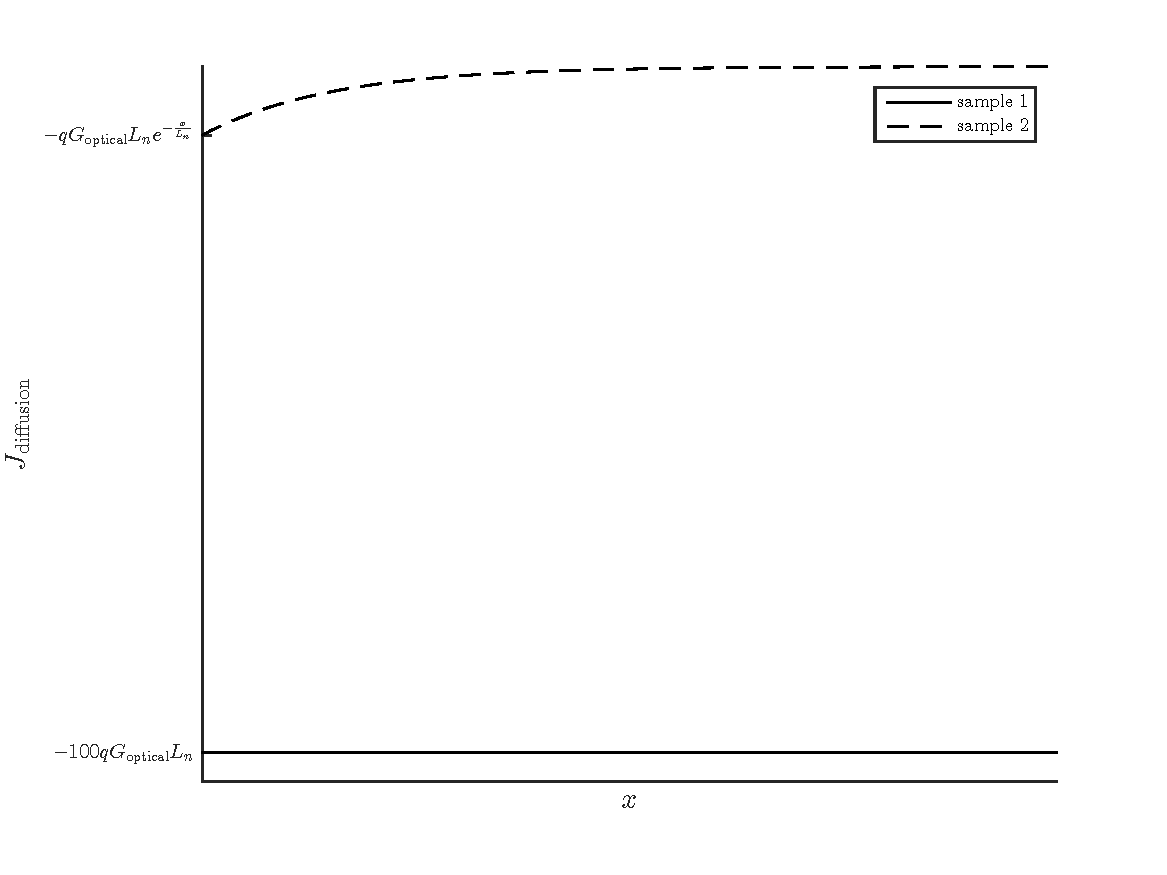
\includegraphics[width = 0.8\textwidth]{plot2.pdf}
			\end{figure}
	\end{enumerate}
\end{solution}

\begin{question}
	Two ends of a uniformly doped N-types silicon bar, of length $L$, are simultaneously illuminated so as to create $\gamma N_D$ excess holes at both $x = 0$ and $x = L$, i.e.,
	\begin{align*}
		\hat{p}_n(0) & = \gamma N_D \\
		\hat{p}_n(L) & = \gamma N_D
	\end{align*}
	where $\gamma = 10^{-3}$.\\
	Light is absorbed only at $x = 0$ and $x = L$, and no light penetrates into the interior of the bar, i.e. for $0 < x < L$, $G_{\text{optical}} = 0$.\\
	Assume that the illumination is steady state, the temperature is $300 \kelvin$, $N_D >> n_i$ and that the bar is long, i.e. $L >> L_n,L_p$.
	\begin{enumerate}
		\item
			Is the carrier generation inside this material low level injection?
			Explain your answer.
		\item
			Sketch the general form of the excess concentration profile $\hat{p}(x)$ across the bar.
		\item
			Write the differential equation from which we can find the solution of $\hat{p}(x)$, and the boundary conditions for this problem.
	\end{enumerate}
\end{question}

\begin{solution}
	\begin{enumerate}[leftmargin=*]
		\item
			\begin{align*}
				n_0 & = N_D
			\end{align*}
			Therefore,
			\begin{align*}
				p_0 & = \frac{{n_i}^2}{N_D} \\
                                    & = \frac{10^{20}}{N_D}
			\end{align*}
			Therefore,
			\begin{align*}
				\hat{p}(0) & = \gamma N_D \\
                                           & = 10^{-3} N_D
			\end{align*}
			Therefore,
			\begin{align*}
				\hat{p}(0) & < N_D \\
				\hat{p}(L) & < N_D
			\end{align*}
			For $0 < x < L$,
			\begin{align*}
				\hat{p}(x) & < \hat{p}(0)
			\end{align*}
			Therefore,
			\begin{align*}
				\hat{p} & < N_D
			\end{align*}
			Therefore, the carrier  generation is low level injection.
		\item
			\begin{figure}[H]
				\centering
				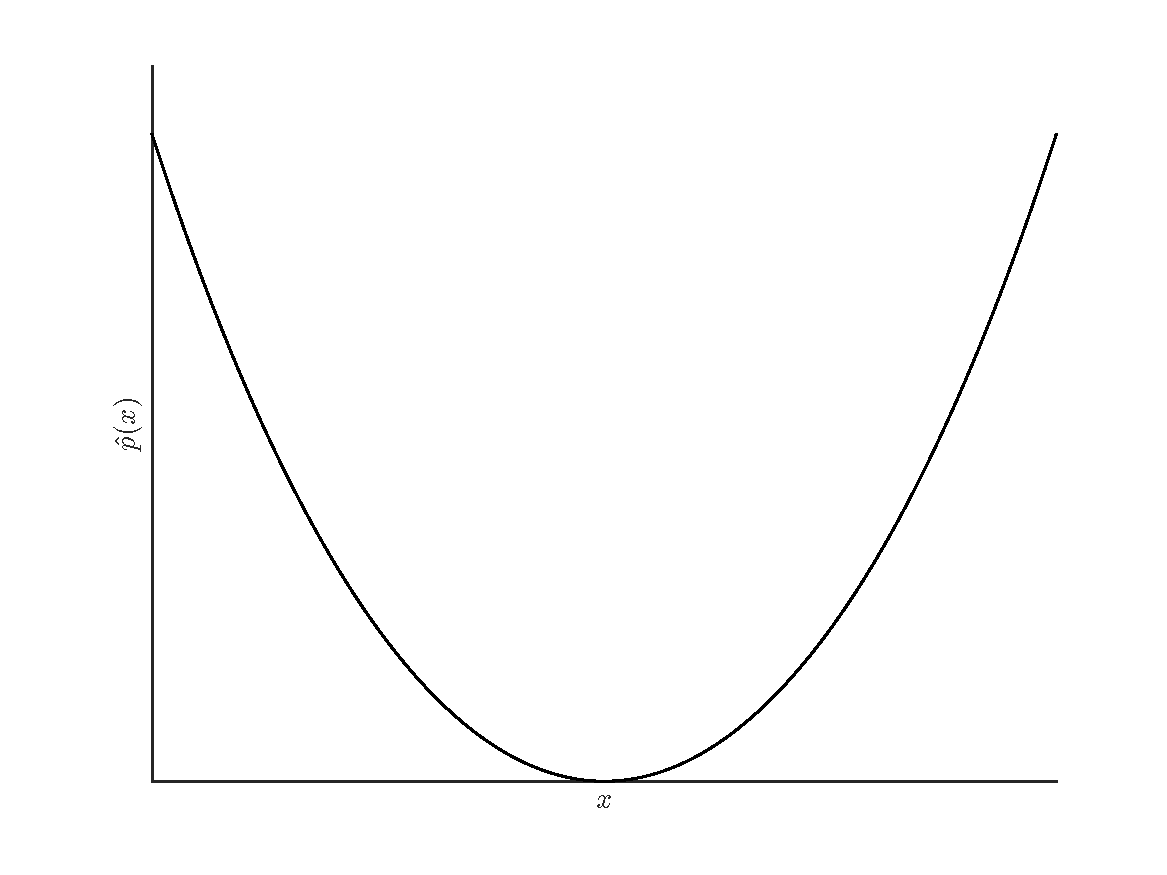
\includegraphics[width = 0.8\textwidth]{plot4.pdf}
			\end{figure}
		\item
			\begin{align*}
				\dpd{\hat{p}(x,t)}{t} & = -\frac{1}{q} \dpd{J_p(x,t)}{x} + G_{\text{optical}} - \frac{\hat{p}(x,t)}{\tau_p}     \\
				\therefore 0          & = -\frac{1}{q} \dpd{J_p(x,t)}{x} - \frac{\hat{p}(x,t)}{\tau_p}                          \\
                                                      & = -\frac{1}{q} \dpd{}{x}\left( -q D_p \dpd{\hat{p}}{x} \right) - \frac{\hat{p}}{\tau_p} \\
                                                      & = \dpd[2]{\hat{p}}{x} - \frac{\hat{p}}{\tau_p}
			\end{align*}
	\end{enumerate}
\end{solution}

\begin{question}
	\begin{enumerate}
		\item
			Consider the $n$th eigenfunction of the one-dimensional harmonic oscillator.
			Using the lowering and raising operators, calculate the following
			\begin{enumerate}
				\item $\langle x \rangle$
				\item $\langle p \rangle$
				\item $\left\langle x^2 \right\rangle$
				\item $\left\langle p^2 \right\rangle$
				\item $\sigma_x$
				\item $\sigma_p$
			\end{enumerate}
			Verify that the uncertainty principle is satisfied.
		\item
			Consider a particle of mass $m$ in the following potential.
			\begin{align*}
				V(x) & = \frac{1}{2} m \omega^2 x^2 + \frac{1}{2} \hbar \omega
			\end{align*}
			Hint: Look at the answer to Question 2 in Homework 5.
			\begin{enumerate}
				\item
					What is the spacing in the ladder of eigenvalues of the energy operator for this potential?
				\item
					What is the lowest possible energy value?
					Write an expression for the energy of the $n$th eigenfunction in this potential.
				\item
					What is the eigenfunction corresponding to the lowest possible energy?
			\end{enumerate}
	\end{enumerate}
\end{question}

\begin{solution}
	\begin{enumerate}[leftmargin=*]
		\item
			\begin{enumerate}[leftmargin=*]
				\item
					\begin{align*}
						\langle x \rangle & = \int\limits_{-\infty}^{\infty} {\psi_n}^* x \psi_n \dif x \\
                                                                  & = \sqrt{\frac{\hbar}{2 m \omega}} \int\limits_{-\infty}^{\infty} {\psi_n}^* \left( \hat{a}_+ + \hat{a}_- \right) \psi_n \dif x
					\end{align*}
					Therefore, solving,
					\begin{align*}
						\langle x \rangle & = 0
					\end{align*}
				\item
					\begin{align*}
						\langle p \rangle & = \int\limits_{-\infty}^{\infty} {\psi_n}^* \hat{p} \psi_n \dif x \\
                                                                  & = \sqrt{\frac{\hbar}{2 m \omega}} \int\limits_{-\infty}^{\infty} {\psi_n}^* \left( \hat{a}_+ - \hat{a}_- \right) \psi_n \dif x
					\end{align*}
					Therefore, solving,
					\begin{align*}
						\langle p \rangle & = 0
					\end{align*}
				\item
					\begin{align*}
						\left\langle x^2 \right\rangle & = \int\limits_{-\infty}^{\infty} {\psi_n}^* x^2 \psi_n \dif x \\
                                                                               & = \sqrt{\frac{\hbar}{2 m \omega}} \int\limits_{-\infty}^{\infty} {\psi_n}^* \left( \hat{a}_+ + \hat{a}_- \right) \left( \hat{a}_+ + \hat{a}_- \right) \psi_n \dif x
					\end{align*}
					Therefore, solving,
					\begin{align*}
						\left\langle x^2 \right\rangle & = \frac{\hbar}{2 m \omega} (2 n + 1)
					\end{align*}
					\begin{align*}
						\left\langle x^2 \right\rangle & = \int\limits_{-\infty}^{\infty} {\psi_n}^* \hat{p}^2 \psi_n \dif x \\
                                                                               & = \sqrt{\frac{\hbar}{2 m \omega}} \int\limits_{-\infty}^{\infty} {\psi_n}^* \left( \hat{a}_+ - \hat{a}_- \right) \left( \hat{a}_+ - \hat{a}_- \right) \psi_n \dif x
					\end{align*}
					Therefore, solving,
					\begin{align*}
						\left\langle p^2 \right\rangle & = \frac{\hbar m \omega}{2} (2 n + 1)
					\end{align*}
				\item
					\begin{align*}
						\sigma_x & = \sqrt{\left\langle x^2 - \right\rangle - \langle x \rangle^2} \\
                                                         & = \sqrt{\frac{\hbar}{2 m \omega} (2 n + 1)}
					\end{align*}
				\item
					\begin{align*}
						\sigma_p & = \sqrt{\left\langle p^2 - \right\rangle - \langle p \rangle^2} \\
                                                         & = \sqrt{\frac{\hbar}{2 m \omega} (2 n + 1)}
					\end{align*}
			\end{enumerate}
			Therefore,
			\begin{align*}
				\sigma_x \sigma_p            & = \frac{\hbar}{2 m \omega} (2 n + 1) \\
				\therefore \sigma_x \sigma_p & \ge \frac{\hbar}{2}
			\end{align*}
			Therefore, the uncertainty principle is satisfied.
		\item
			\begin{enumerate}[leftmargin=*]
				\item
					Let $\psi(x)$ be a solution to
					\begin{align*}
						V_1(x) & = \frac{1}{2} m \omega^2 x^2
					\end{align*}
					Therefore, as $\frac{1}{2} \hbar \omega$ is constant, $\psi(x)$ is also a solution to
					\begin{align*}
						V(x) & = \frac{1}{2} m \omega^2 x^2 + \frac{1}{2} \hbar \omega
					\end{align*}
					Therefore, the spacing in the ladder of the eigenvalues of the energy operator for this potential is the same as a standard quantum harmonic oscillator, i.e. $\hbar \omega$.
				\item
					As the eigenfunctions of $V(x)$ and $V_1(x)$ are common,
					\begin{align*}
						\psi_0(x) & = \left( \frac{m \omega}{\hbar \pi} \right)^{\frac{1}{4}} e^{-\frac{m \omega}{2 \hbar} x^2}
					\end{align*}
					Therefore, the eigenvalues are the same as for a quantum harmonic oscillator, with $\frac{1}{2} \hbar \omega$ added.
					Therefore,
					\begin{align*}
						E_0 & = \frac{1}{2} \hbar \omega + \frac{1}{2} \hbar \omega \\
                                                    & = \hbar \omega
					\end{align*}
					Therefore,
					\begin{align*}
						E_n & = (n + 1) \hbar w
					\end{align*}
			\end{enumerate}
	\end{enumerate}
\end{solution}

\begin{question}
	\begin{enumerate}
		\item
			Show the following commutation relations.
			\begin{enumerate}
				\item $\left[ \hat{L}_z,\hat{L}_+ \right] = \hbar \hat{L}_+$
				\item $\left[ \hat{L}_z,\hat{L}_- \right] = -\hbar \hat{L}_-$
				\item $\left[ \hat{L}^2,\hat{L}_+ \right] = 0$
				\item $\left[ \hat{L}^2,\hat{L}_- \right] = 0$
			\end{enumerate}
			where
			\begin{align*}
				\hat{L}_- & = \hat{L}_x - i \hat{L}_y \\
				\hat{L}_+ & = \hat{L}_x + i \hat{L}_y
			\end{align*}
		\item
			Explain what $\hat{L}_-$ does to an eigenfunction of the angular momentum in the $z$ direction, i.e. $\hat{L}_z$.
			Hint: Apply $\hat{L}_z$ on $\hat{L}_- Y_{l m}$, where $Y_{l m}$ is an eigenfunction of $\hat{L}_z$, i.e. $\hat{L}_z Y_{l m} = \hbar m Y_{l m}$.
		\item
			Explain what $\hat{L}_-$ does to an eigenfunction of the total angular momentum squared operator, i.e. $\hat{L}^2$.
			Hint: Apply $\hat{L}^2$ on $\hat{L}_- Y_{l m}$, where $Y_{l m}$ is an eigenfunction of $\hat{L}^2$, i.e. $\hat{L}^2 Y_{l m} = \hbar^2 l (l + 1) Y_{l m}$.
	\end{enumerate}
\end{question}

\begin{solution}
	\begin{enumerate}[leftmargin=*]
		\item
			\begin{enumerate}[leftmargin=*]
				\item
					\begin{align*}
						\left[ \hat{L}_z,\hat{L}_+ \right] & = \hat{L}_z \hat{L}_+ - \hat{L}_+ \hat{L}_z                                 \\
                                                                                   & = \left[ \hat{L}_z,\hat{L}_x \right] + i \left[ \hat{L}_z,\hat{L}_y \right] \\
                                                                                   & = i \hbar \hat{L}_y + i \left( -i \hbar \hat{L}_x \right)                   \\
                                                                                   & = \hbar \left( \hat{L}_x + i \hat{L}_y \right)                              \\
                                                                                   & = \hbar \hat{L}_+
					\end{align*}
				\item
					\begin{align*}
						\left[ \hat{L}_z,\hat{L}_- \right] & = \hat{L}_z \hat{L}_- - \hat{L}_- \hat{L}_z                                 \\
                                                                                   & = \left[ \hat{L}_z,\hat{L}_x \right] - i \left[ \hat{L}_z,\hat{L}_y \right] \\
                                                                                   & = i \hbar \hat{L}_y - i \left( -i \hbar \hat{L}_x \right)                   \\
                                                                                   & = -\hbar \left( \hat{L}_x - i \hat{L}_y \right)                             \\
                                                                                   & = -\hbar \hat{L}_+
					\end{align*}
				\item
					\begin{align*}
						\left[ \hat{L}^2,\hat{L}_+ \right] & = \left[ \hat{L}^2,\hat{L}_x + i \hat{L}_y \right]                          \\
                                                                                   & = \left[ \hat{L}^2,\hat{L}_x \right] + i \left[ \hat{L}^2,\hat{L}_y \right] \\
                                                                                   & = 0 + 0                                                                     \\
                                                                                   & = 0
					\end{align*}
				\item
					\begin{align*}
						\left[ \hat{L}^2,\hat{L}_- \right] & = \left[ \hat{L}^2,\hat{L}_x - i \hat{L}_y \right]                          \\
                                                                                   & = \left[ \hat{L}^2,\hat{L}_x \right] - i \left[ \hat{L}^2,\hat{L}_y \right] \\
                                                                                   & = 0 - 0                                                                     \\
                                                                                   & = 0
					\end{align*}
			\end{enumerate}
		\item
			Let $Y_{l m}$ be an eigenfunction of $\hat{L}_z$, with eigenvalue $m$.
			\begin{align*}
				\hat{L}_z \hat{L}_- Y_{l m} & = \left( \left[ \hat{L}_z,\hat{L}_- \right] + \hat{L}_- \hat{L}_z \right) Y_{l m} \\
                                                            & = \left( -\hbar \hat{L}_- + \hat{L}_- m \hbar \right) Y_{l m}                     \\
                                                            & = \hbar (m - 1) \hat{L}_- Y_{l m}
			\end{align*}
			Therefore, $\hat{L}_- Y_{l m}$ is an eigenfunction of $\hat{L}_z$ with eigenvalue $\hbar (m - 1)$.
		\item
			Similarly, let $Y_{l m}$ be an eigenfunction of $\hat{L}_z$, with eigenvalue $\hbar l (l + 1)$.
			\begin{align*}
				\hat{L}^2 \hat{L}_- Y_{l m} & = \hbar^2 l (l + 1) \hat{L}_- Y_{l m}
			\end{align*}
			Therefore, $\hat{L}_- Y_{l m}$ is also an eigenfunction of $\hat{L}^2$, with the same eigenvalue.
	\end{enumerate}
\end{solution}

\end{document}
